\documentclass[11pt]{article}
\usepackage{fancyhdr}
\usepackage{tocloft}
\usepackage{graphicx}
\usepackage{calc}
\usepackage{amssymb}
\usepackage{color}
\usepackage[sc]{mathpazo}
\usepackage{url}
\usepackage{ifpdf}
\usepackage{bbding}
\usepackage{caption}
\usepackage{framed}
\usepackage{xcolor}
\usepackage{float}
\usepackage{wrapfig}
\usepackage{sidecap}
\usepackage{multirow}
\linespread{1.0}
\oddsidemargin=0pt
\evensidemargin=0pt
\textwidth=6.5in
\topmargin=0pt
\headheight=0pt
\headsep=0pt
\textheight=9in
\setlength{\parindent}{0.25cm}
\newcommand\secfont{\fontfamily{cmss}\selectfont}%\textwidth 5.5truein
\newcommand\pifheading[1]{\noindent{\secfont\textbf{#1}:}}
\newcommand\yr{2016}
\def\lo{
\mathrel{\raise.3ex\hbox{$<$}\mkern-14mu\lower0.6ex\hbox{$\sim$}}
}
\def\hi{
\mathrel{\raise.3ex\hbox{$>$}\mkern-14mu\lower0.6ex\hbox{$\sim$}}
}

\textwidth = 6.5 in
\textheight = 9 in
\oddsidemargin = -0.00 in
\evensidemargin = +0.05 in
\topmargin = 0 in
\headheight = 0.0 in
\headsep = 0.0 in
\parskip = 0.05in

\newcommand\registered{{\ooalign{\hfil\raise .00ex\hbox{\scriptsize R}\hfil\crcr\mathhexbox20D}}}

%% Define a new 'leo' style for the package that will use a smaller font.
\makeatletter
\def\url@leostyle{%
  \@ifundefined{selectfont}{\def\UrlFont{\sf}}{\def\UrlFont{\small\ttfamily}}}
\makeatother
%% Now actually use the newly defined style.
\urlstyle{leostyle}
\newcommand\checkme[1]{\textcolor{blue}{\textbf{#1}}}
\newcounter{hours}\newcounter{minutes}
\newcommand\printtime{\setcounter{hours}{\time/60}\setcounter{minutes}{\time - \value{hours}*60}\thehours :\theminutes}
\newenvironment{packed_item}{
\begin{itemize}
 \setlength{\itemsep}{1pt}
 \setlength{\parskip}{0pt}
 \setlength{\parsep}{0pt}
}{\end{itemize}}

\newenvironment{packed_enum}{
\begin{enumerate}
 \setlength{\itemsep}{1pt}
 \setlength{\parskip}{0pt}
 \setlength{\parsep}{0pt}
}{\end{enumerate}}

\newenvironment{box_list}{
\begin{itemize}
 \setlength{\itemsep}{3pt}
 \setlength{\parskip}{0pt}
 \setlength{\parsep}{0pt}
}{\end{itemize}}

\newenvironment{packed_list}{
\begin{list}{\labelitemi}{\leftmargin=1em}
 \setlength{\itemsep}{3pt}
 \setlength{\parskip}{0pt}
 \setlength{\parsep}{0pt}
}{\end{list}}

\renewenvironment{quote}{%
  \list{}{%
    \leftmargin10pt   % this is the adjusting screw
    \rightmargin\leftmargin
  }
  \item\relax
}
{\endlist}

% definition of a new float type (refer to the caption package documentation)
\DeclareCaptionType{boxcaption}[Box]
\captionsetup[boxcaption]{position=top,labelfont=bf}

% definition of a shaded-like environment (see framed.sty)
\newenvironment{shadedframe}
  {\def\FrameCommand{\setlength\fboxsep{10pt}\fcolorbox{black}{shadecolor}}%
    \MakeFramed {\advance\hsize-\width \FrameRestore}}%
{\endMakeFramed}

\newenvironment{shadedbox}{%
  \def\FrameCommand{\colorbox{shadecolor}}%
  \MakeFramed {\FrameRestore}}%
 {\endMakeFramed}

% main environment
% syntax: \begin{myenv}{placement-specifiers}{color}{width}...\end{myenv}
\newenvironment{boxenv}[3]
  {\colorlet{shadecolor}{#2}%
    \begin{boxcaption}[#1]%
    \noindent\begin{minipage}{#3}
      \begin{shadedframe}
      }
  {\end{shadedframe}\end{minipage}\end{boxcaption}}

 % TOC
\usepackage{enumerate}
\begin{document}


\begin{figure}
  
\includegraphics[width=\linewidth/3]{title}
  \label{fig:title}
\end{figure}


\title{Lab Report 9: Digital Electronics The Basics}


\author{Yuezhe Yao}

%\institute{Syracuse University}



\maketitle

\begin{abstract}
In this lab, we utilized LabVIEW and the digital functions of our DAQ card to learn some of the basics of digital electronics and operate several important digital components.      
\end{abstract}

\medskip

\begingroup
\let\clearpage\relax
\tableofcontents
\endgroup

\medskip
\medskip

\section{Learning Objectives}


To become familiar with basic digital concepts and terminology 

To become familiar with the digital input/output (I/O) functions of LabVIEW and the NI USB-6003

To learn about important digital circuit elements like gates, flip-flops, timers, counters, and registers

To gain appreciation of how digital circuits shape our modern world

\section{Activity I - Basic Introduction to Digital Concepts \& Termin
ology}


For 3-input NAND, except the condition when all the 3 inputs are 1, the output would be 0 then. Otherwise the output would be 1.

A \quad B  \quad  C  \quad X

1  \quad\,  1 \quad 1  \quad\,   0

otherwise \quad \ \, 1

\vbox{}

For 2-input XOR

A \quad B   \quad \ X

0  \quad\,  0 \quad\,   0

0  \quad\,  1 \quad\,   1

1  \quad\,  0 \quad\,   1

1  \quad\,  1 \quad\,   0

\vbox{}

Yes we were able to reproduce these tables.


\section{Activity II - Digital I/O with LabVIEW and the PCI-6023/24E}


\begin{figure}[H]
 \begin{center}
  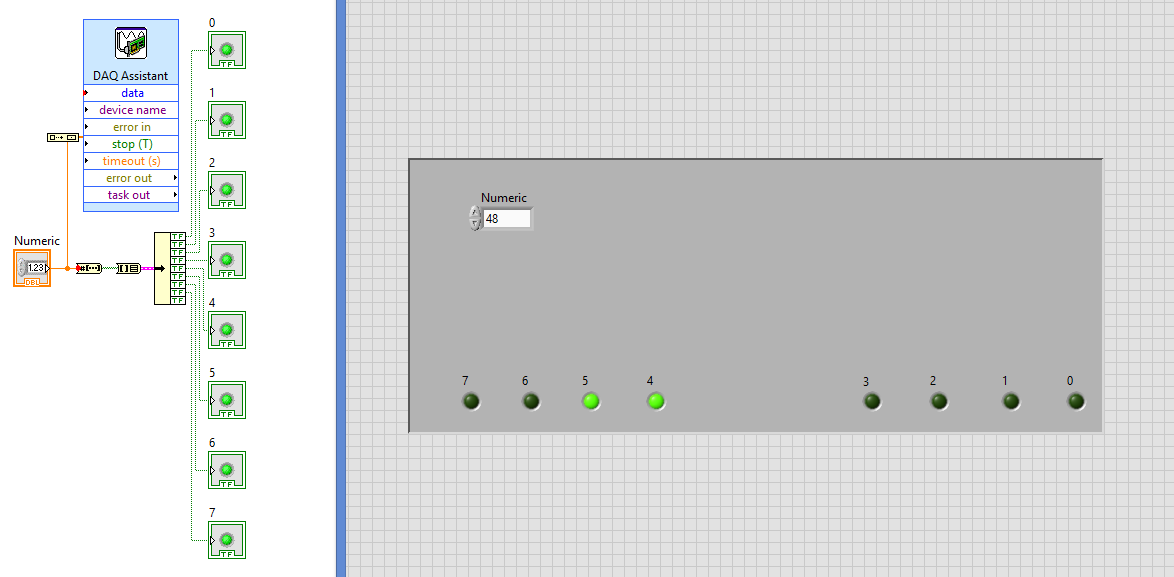
\includegraphics[width=\linewidth/1]{act2_2}
  \caption{The front panel and block diagram of the output of all integers from 1 to 255.}
  \label{fig:act2_2}
 \end{center}
\end{figure}

\begin{figure}[H]
 \begin{center}
  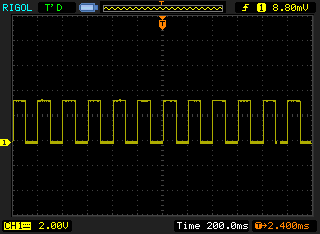
\includegraphics[width=\linewidth/2]{act2_2b}
  \caption{The output of a square TTL wave.}
  \label{fig:act2_2b}
 \end{center}
\end{figure}

\begin{figure}[H]
 \begin{center}
  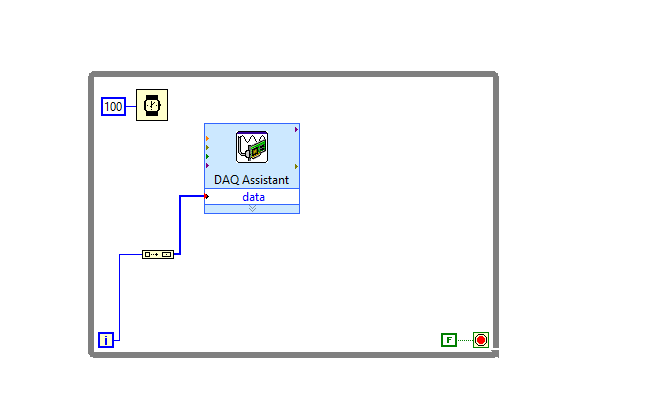
\includegraphics[width=\linewidth/2]{act2_3b}
  \caption{The block diagram of the output of a square TTL wave.}
  \label{fig:act2_3b}
 \end{center}
\end{figure}

\begin{figure}[H]
 \begin{center}
  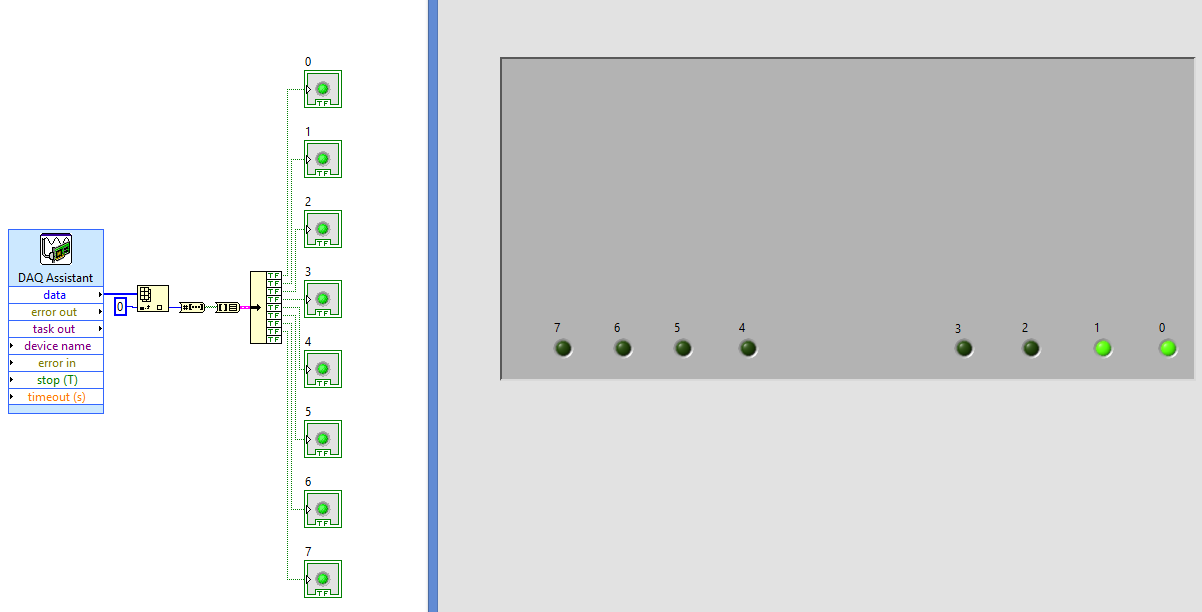
\includegraphics[width=\linewidth/2]{act2_4}
  \caption{The front panel and block diagram of the display of the logic levels on LED indicators.}
  \label{fig:act2_4}
 \end{center}
\end{figure}


\section{Activity III - The 2-Bit Full Adder and Subtractor}


\begin{figure}[H]
 \begin{center}
  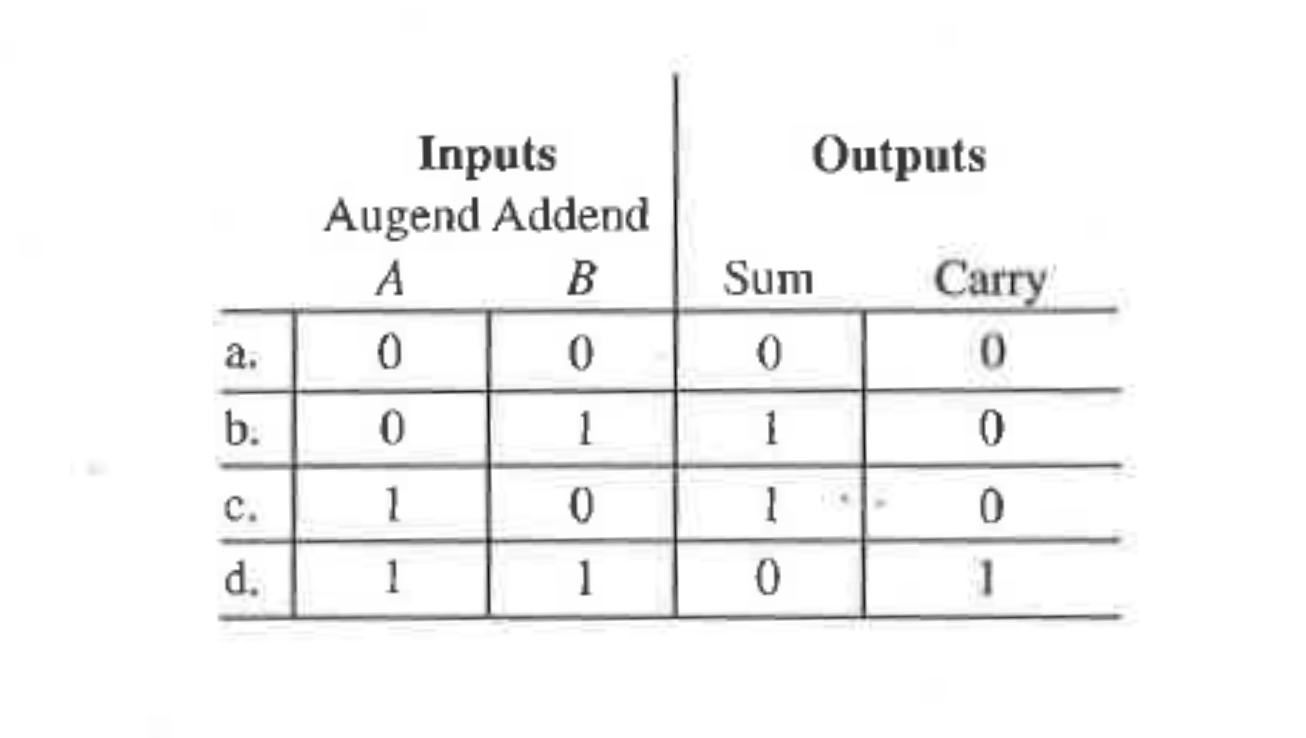
\includegraphics[width=\linewidth/2]{act3}
  \caption{The truth table the full adder.}
  \label{fig:act3}
 \end{center}
\end{figure}

Yes our circuit operated in the manner that we expected.


\section{Activity IV - Flip-Flops}

\begin{figure}[H]
 \begin{center}
  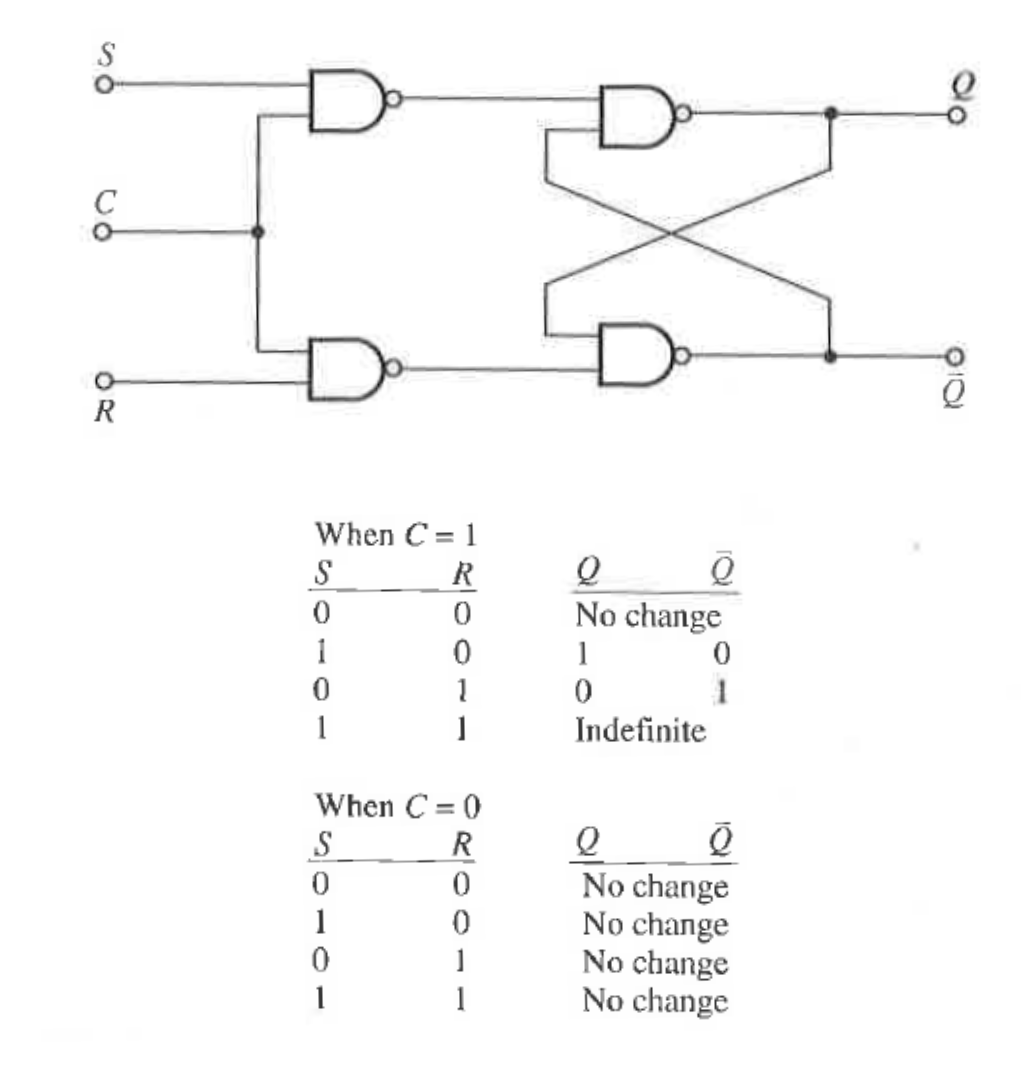
\includegraphics[width=\linewidth/2]{act4rsff}
  \caption{RSFF.}
  \label{fig:act4rsff}
 \end{center}
\end{figure}

For the clocked RSFF

Everything went well and we successfully get the right truth table

\begin{figure}[H]
 \begin{center}
  \includegraphics[width=\linewidth/1]{act5acapac100Hz}
  \caption{The front panel of the half-wave rectifier with the capacitor(100Hz).}
  \label{fig:act5acapac100Hz}
 \end{center}
\end{figure}

\begin{figure}[H]
 \begin{center}
  \includegraphics[width=\linewidth/1]{act5anocapac100Hz}
  \caption{The front panel of the half-wave rectifier without the capacitor(100Hz).}
  \label{fig:act5anocapac100Hz}
 \end{center}
\end{figure}

\begin{figure}[H]
 \begin{center}
  \includegraphics[width=\linewidth/1]{act5b10Hz4v-6v}
  \caption{The front panel of the diode clipper(V1=4V, V2=-6V).}
  \label{fig:act5b10Hz4v-6v}
 \end{center}
\end{figure}

\begin{figure}[H]
 \begin{center}
  \includegraphics[width=\linewidth/1]{act5c10Hzcapac}
  \caption{The front panel of the full-wave rectifier with the capacitor(10Hz).}
  \label{fig:act5c10Hzcapac}
 \end{center}
\end{figure}

\begin{figure}[H]
 \begin{center}
  \includegraphics[width=\linewidth/1]{act5c10Hznocapac}
  \caption{The front panel of the full-wave rectifier without the capacitor(10Hz).}
  \label{fig:act5c10Hznocapac}
 \end{center}
\end{figure}



\end{document}
